\newcommand{\econtexRoot}{.}
% The \commands below are required to allow sharing of the same base code via Github between TeXLive on a local machine and ShareLaTeX.  This is an ugly solution to the requirement that custom LaTeX packages be accessible, and that ShareLaTeX seems to ignore symbolic links (even if they are relative links to valid locations)
\providecommand{\econtex}{\econtexRoot/texmf-local/tex/latex/econtex}
\providecommand{\econtexSetup}{\econtexRoot/texmf-local/tex/latex/econtexSetup}
\providecommand{\econtexShortcuts}{\econtexRoot/texmf-local/tex/latex/econtexShortcuts}
\providecommand{\econtexBibMake}{\econtexRoot/texmf-local/tex/latex/econtexBibMake}
\providecommand{\econtexBibStyle}{\econtexRoot/texmf-local/bibtex/bst/econtex}
\providecommand{\notes}{\econtexRoot/texmf-local/tex/latex/handout}
\providecommand{\handoutSetup}{\econtexRoot/texmf-local/tex/latex/handoutSetup}
\providecommand{\handoutShortcuts}{\econtexRoot/texmf-local/tex/latex/handoutShortcuts}
\providecommand{\handoutBibMake}{\econtexRoot/texmf-local/tex/latex/handoutBibMake}
\providecommand{\handoutBibStyle}{\econtexRoot/texmf-local/bibtex/bst/handout}

  
\documentclass[titlepage]{\econtex}\newcommand{\texname}{BPP_PSID_TimeAgg}

\usepackage{\econtexSetup}\usepackage{\econtexShortcuts}

\usepackage[nolists,nomarkers,tablesonly]{endfloat}

\hypersetup{pdfauthor={Edmund Crawley <ecrawle2@jhu.edu>},
            pdftitle={Consumption Inequality and Partial Insurance: A Correction for Time Aggregation},
            pdfsubject={Consumption Inequality and Partial Insurance: A Correction for Time Aggregation},
            pdfkeywords={Consumption, Insurance; JEL: D12, D31, D91, E21},
            pdfproducer = {LaTeX with hyperref and thumbpdf},
            pdfcreator = {pdflatex}
            }

\newlength{\defbaselineskip}
\setlength{\defbaselineskip}{\baselineskip}
\newcommand{\setlinespacing}[1]%
           {\setlength{\baselineskip}{#1 \defbaselineskip}}

\newlength\TableWidth

\usepackage{titlesec}

\setcounter{secnumdepth}{4}

\titleformat{\paragraph}
{\sffamily\mdseries\normalsize}{\theparagraph}{1em}{}
\titlespacing*{\paragraph}
{0pt}{3.25ex plus 1ex minus .2ex}{1.5ex plus .2ex}


\begin{document}\bibliographystyle{\econtexBibStyle}

\newcolumntype{d}[1]{D{.}{.}{#1}}
\providecommand{\perc}[1]{\widetilde{#1}}

\begin{verbatimwrite}{\jobname.title}
Sticky Expectations and Consumption Dynamics
\end{verbatimwrite}

\hfill{\tiny \jobname}

\title{Consumption Inequality and Partial Insurance: 
A Correction for Time Aggregation}

\author{
  Edmund Crawley \\ {\small Johns Hopkins University and Danmarks Nationalbank}
}


\keywords{Consumption, Insurance}
\jelclass{D12, D31, D91, E21}
% \aspublished{Final version as published in [].}

\maketitle
%\maketitleWithForcedDate{July 1, 2010}

\begin{abstract}
  \opt{JournalFormatting}{\doublespacing} The extent to which households are able to insure themselves against shocks to their income plays a key role in business cycle dynamics. In an influential paper making use of the covariance structure in PSID data \cite{blundell_consumption_2008} (BPP) find almost full insurance against transitory shocks to income. This result diverges from the majority of the literature aimed at measuring the marginal propensity to consume that finds consumption responds sharply to transitory income shocks. In this paper I show that the discretization of time in the BPP model is far from a benign assumption. Allowing shocks to arrive in continuous time throughout each year changes the covariance structure of the model. I repeat the minimum distance estimation exercise matching moments from the equivalent continuous time model and find the pass through from income to consumption for transitory shocks increases from around 5\% to 24\%.
\end{abstract}

\begin{authorsinfo}
\name{Crawley: Department of Economics, Johns Hopkins University, Baltimore, MD, \href{mailto:ecrawle2@jhu.edu}{\texttt{ecrawle2@jhu.edu}}, Phone:  (917) 374 2942}
\end{authorsinfo}
\thanks{Thanks to...}

\titlepagefinish
\setcounter{page}{1}

\pagebreak

\provideboolean{SlidesInText}
\setboolean{SlidesInText}{true}

\section{Introduction}
\cite{blundell_consumption_2008} 
\cite{working_note_1960}
\cite{kaplan_how_2010} ``we argue that the BPP insurance coefficients should become central in quantitative macroeconomics"
\subsection{Estimates of the Marginal Propensity to Consume}
Show the BPP estimate is far away from consensus. \cite{jappelli_consumption_2010}

\subsection{Applications of the BPP methodology}
\cite{violante_wealthy_2014}
\cite{auclert_monetary_2015}

\section{The Time Aggregation Problem}
The results of this paper derive from the insight of \cite{working_note_1960}. He was the first to note that the use of averages in time series data can results in correlations that are not present in the original series. Intuition on this result can be obtained by thinking about a random walk in continuous time (such as a Weiner process $W_t$) where we are only able to observe a discrete series $\bar{W}_T$ for $T \in \{1,2,3...\}$ corresponding to the mean value of the series between $T-1$ and $T$. If a shock occurs halfway through a period, $\bar{W}_T$ will increase by half the value of the shock and $\bar{W}_{T+1}$ will be expected to be larger than $\bar{W}_T$ by half the value of the shock again. In this way an autocorrelation is induced in the time-aggregated series, even though the underlying series is a pure random walk. In continous time this correlation takes a value of $\frac{1}{6}$.

Once the problem is recognized it is immediately apparent that it may have important implications for the BPP methodology that relies on the covariance structure of income and consumption to identify the insurance coefficients. In this section I first describe the BPP methodology in discrete time as originally proposed. I then illustrate the time-aggregation problem by dividing time up into two sub-periods. Finally I write down an equivalent continuous time model and use it to derive a time-aggregate corrected set of moments to use in the minimum distance estimation.

\subsection{BPP Moments in Discrete Time}
Here I briefly describe the method followed by \cite{blundell_consumption_2008}. For a more detail please refer to their original paper. The core of the model are their assumptions on the income and consumption processes. They assume that (unexplained) income growth for household $i$ follows the process:
\begin{align*}
\Delta y_{i,t} = \zeta_{i,t} + \Delta \nu_{i,t}
\end{align*}
where time is discrete, the permanent shock component $\zeta_{i,t}$ is serially uncorrelated and the transitory shock component $\nu_{i,t}$ follows an MA(q) process. The (unexplained) change in log consumption is assumed to be:
\begin{align*}
\Delta c_{i,t} = \phi_{i,t}\zeta_{i,t} + \psi_{i,t} \nu_{i,t} + \xi_{i,t}
\end{align*}
where $\phi_{i,t}$ and $\psi_{i,t}$ are the \textit{partial insurance} parameters for permanent and transitory shocks respectively. $\xi_{i,t}$ represents unobserved taste shocks. 

Identification of the parameters is achieved by matching the covariance structure of the model with that in the data. In the simple case in which $\nu_{i,t}$ is a random walk (q=0), and assuming stationarity, the two insurance parameters are identified by:
\begin{align}
\phi &= \frac{cov(\Delta c_t, \Delta y_{t-1}+\Delta y_{t}+\Delta y_{t+1})}{cov(\Delta y_t, \Delta y_{t-1}+\Delta y_{t}+\Delta y_{t+1})} \label{perm_ins} \\
\psi &= \frac{cov(\Delta c_t,\Delta y_{t+1})}{cov(\Delta y_t,\Delta y_{t+1})} \label{tran_ins}
\end{align}

\subsection{A Two Sub-Period Example}
This section aims to give intuition to the problem that arises from the discrete time assumption made by BPP. I will calculate the moments \ref{perm_ins} and \ref{tran_ins} but under the assumption that the true process is semi-annual while we only observe the sum of income and consumption every year.

As in BPP the underlying processes for income and consumption growth are:
\begin{align*}
\Delta y_t & = \zeta_t + \varepsilon_t - \varepsilon_{t-1} \\
\Delta c_t & = \phi \zeta_t + \psi \varepsilon_t  \\
\end{align*}
where now $t$ denotes 6-month periods. Summing up (assuming $y_0=c_0=0$) gives:
\begin{align*}
y_t & = \sum_{i=1}^t \zeta_i + \varepsilon_t  \\
c_t & = \phi \sum_{i=1}^t \zeta_i + \psi \sum_{i=1}^t \varepsilon_i  \\
\end{align*}
We observe $y^{obs}_T$ and $c^{obs}_T$ for $T \in \{2,4,6...\}$ (annually) where:
\begin{align*}
y^{obs}_T & = y_T + y_{T-1}  \\
c^{obs}_T & = c_T + c_{T-1}  \\
\end{align*}
Our observed (annual) changes in income and consumption are therefore:
\begin{align*}
\Delta^2 y^{obs}_T & \equiv y^{obs}_T-y^{obs}_{T-2} =  y_T + y_{T-1} - y_{T-2} - y_{T-3} \\
\Delta^2 c^{obs}_T & \equiv c^{obs}_T-c^{obs}_{T-2} =  c_T + c_{T-1} - c_{T-2} - c_{T-3}  \\
\end{align*}
which implies:
\begin{align*}
\Delta^2 y^{obs}_T & = \zeta_T + 2\zeta_{T-1} +\zeta_{T-2} + \varepsilon_T + \varepsilon_{T-1} - \varepsilon_{T-2} - \varepsilon_{T-3} \\
\Delta^2 c^{obs}_T & =  \phi(\zeta_T + 2\zeta_{T-1} +\zeta_{T-2}) + \psi(\varepsilon_T + 2\varepsilon_{T-1} + \varepsilon_{T-2} ) \\
\end{align*}
I can use these to calculate the estimates retrieved by using the identifying moments \ref{perm_ins} and \ref{tran_ins} for the permanent and transitory insurance parameters:
\begin{align}
\mathbb{E} \hat{\phi} &= \frac{cov(\Delta^2 c^{obs}_T,\Delta^2 y^{obs}_{T+2}+\Delta^2 y^{obs}_{T}+\Delta^2 y^{obs}_{T-2})}{cov(\Delta^2 y^{obs}_T,\Delta^2 y^{obs}_{T+2}+\Delta^2 y^{obs}_{T}+\Delta^2 y^{obs}_{T-2})} \nonumber \\
&= \frac{\phi (2var(\zeta_T) + 4var(\zeta_{T-1}) + 2var(\zeta_{T-2})) }{2var(\zeta_T) + 4var(\zeta_{T-1}) + 2var(\zeta_{T-2})  } \nonumber\\
& = \phi	\label{phihat}
\end{align}
\begin{align}
\mathbb{E} \hat{\psi} &= \frac{cov(\Delta^2 c^{obs}_T,\Delta^2 y^{obs}_{T+2})}{cov(\Delta^2 y^{obs}_T,\Delta^2 y^{obs}_{T+2})} \nonumber\\
& = \frac{\phi var(\zeta_T) -\psi(var(\varepsilon_T) + 2var(\varepsilon_{T-1}) )}{ var(\zeta_T) - var(\varepsilon_T) -var(\varepsilon_{T-1}) } \nonumber\\
& = \frac{\phi var(\zeta_T) -3\psi var(\varepsilon_T)  }{ var(\zeta_T) - 2var(\varepsilon_T)  }	\label{psihat}
\end{align}
From equation \ref{phihat} we can see the estimator for the permanent shock insurance parameter is still unbiased, but equation \ref{psihat} shows this is not the case for the transitory shock insurance parameter. To take a simple example consider the permanent income hypothesis with $\phi=1$ and $\psi=0$. Using the annual BPP methodology with a semi-annual shock process would yield a correct estimate of $1$ for $\phi$, but the estimate for $\psi$ would be  $\frac{var(\zeta_T)   }{ var(\zeta_T) - 2var(\varepsilon_T)  }$, a number that could take on almost any value depending on the relative variances of permanent and transitory shocks.

\subsection{Continuous Time Moments in PSID Data}
It should now be clear that assuming a discrete annual time period for the model income and consumption processes will not suffice. In order for the BPP method to give us a reasonable estimate of the transitory shock insurance parameter the model will need to account for the fact that shocks can arrive at any point during the year. In this section I derive the covariance structure of a model that is as close to the original BPP model but derived in continuous time.

In the stationary continuous time model we have two underlying martingale processes (possibly with jumps), $P_t$ and $Q_t$ such that for all $s_1>s_2>s_3>s_4>0$:
\begin{align*}
var(P_{s_1}-P_{s_2})=(s_1-s_2)\sigma_P^2 \\
cov(P_{s_1}-P_{s_2},P_{s_3}-P_{s_4}) = 0 \\
P_s = 0 \qquad \text{if } s<0
\end{align*}
and similarly for $Q_t$. Instantaneous income in a period $dt$ is given by:
\begin{align}
y_t dt = \Big( \int_{0}^{t}dP_s \Big) dt  +dQ_t \label{income_process}
\end{align}
so that $P_t$ and $Q_t$ are exactly analogous to the permanent and transitory shocks in the discrete time model (with $q=0$ in the MA($q$) transitory component - see appendix ***** to relax this assumption). Keeping with the assumption that consumption is a random walk with insurance parameters $\phi$ and $\psi$, instantaneous consumption is given by
\begin{align}
c_t dt = \phi \Big( \int_{0}^{t} dP_s  \Big) dt +\psi\Big( \int_{0}^{t}dQ_s\Big) dt +\Big( \int_{0}^{t}d\xi_s\Big) dt \label{consumption_process}
\end{align}
where $\xi_t$ is also a martingale process similar to $P_t$ and $Q_t$ and represents innovations in consumption (taste shocks) that are independent of those in income (c.f. $\xi_{t}$ in BPP).

Equations \ref{income_process} and \ref{consumption_process} give the instantaneous income and consumption process in continuous time. To bring this model to the covariance matrix in the PSID data it is necessary to calculate the model implied covariance matrix, which requires paying attention to exactly what is being measured in the PSID data. For income, the survey asks about total income in the previous calendar year. In the model this is equivalent to the quantity $\bar{y}_T$ where
\begin{align*}
\bar{y}_T = \int_{T-1}^{T} y_t dt
\end{align*}
for $T \in \{1,2,3...\}$. BPP use questions about food consumption to impute the level of total consumption. The questionnaire asks about food consumption in a typical week, but unfortunately the timing of this `typical week' is less clear. The questionnaire is usually given at the end of March in the following year. See \cite{altonji_testing_1987} and \cite{hall_sensitivity_1982} for differing views. Here I will assume the `typical week' occurs exactly at the end of the calendar year, so it measures the snapshot of consumption $c_T$ for $T \in \{1,2,3...\}$. In appendix ***** I show that the data does not fit an alternative assumption that the `typical week' is an average for the previous calendar year.

The covariance structure is based on observable annual changes in income and consumption:
\begin{align}
\Delta \bar{y}_T &= \int_{T-1}^{T} y_t dt - \int_{T-2}^{T-1} y_t dt \nonumber \\ 
&= \int_{T-1}^{T} \int_{0}^{t}dP_s dt -\int_{T-2}^{T-1} \int_{0}^{t}dP_s dt +  \int_{T-1}^{T} dQ_t -\int_{T-2}^{T-1} dQ_t \nonumber \\
&= \int_{T-1}^{T} \int_{t-1}^{t}dP_s dt +  \int_{T-1}^{T} dQ_t -\int_{T-2}^{T-1} dQ_t \nonumber \\
&= \Big(\int_{T-2}^{T-1} (s-(T-2))dP_s  + \int_{T-1}^{T} (T-s)dP_s \Big) \nonumber \\
& \qquad + \Big(\int_{T-1}^{T} dQ_t -\int_{T-2}^{T-1} dQ_t \Big) \label{deltay}
\end{align}
\begin{align}
\Delta c_T &= c_T - c_{T-1} \nonumber  \\
&= \phi  \int_{T-1}^{T} dP_s  +\psi \int_{T-1}^{T}dQ_s +\int_{T-1}^{T}d\xi_s  \label{deltac}
\end{align}
The key moments of interest are the covariances of consumption change with differing lags of income change:
\begin{align}
cov(\Delta c_T^*, \Delta \bar{y}_T) &=  \mathbb{E} \Big( \phi \int_{T-1}^{T} (T-s) dP_s dP_s + \psi \int_{T-1}^{T} dQ_s dQ_s \Big) \nonumber \\
&= \frac{1}{2} \phi \sigma^2_P + \psi \sigma^2_Q \\
cov(\Delta c_T^*, \Delta \bar{y}_{T+1}) &=  \mathbb{E} \Big( \phi \int_{T-1}^{T} (s-(T-1)) dP_s dP_s - \psi \int_{T-1}^{T} dQ_s dQ_s \Big) \nonumber \\
&= \frac{1}{2} \phi \sigma^2_P - \psi \sigma^2_Q \\
cov(\Delta c_T^*, \Delta \bar{y}_{T-1}) &= 0 \\
cov(\Delta c_T^*, \Delta \bar{y}_{S}) &= 0 \qquad \forall S,T \text{ such that }|S-T| >1 
\end{align}
For the baseline model I relax the assumption of stationarity and also add measurement error in consumption making exactly analogous assumptions to those in the original BPP paper. The full set of moments are calculated in appendix *********.
\section{The Evidence}
Table \ref{table:ReplicationTable} replicates the first 3 columns from Table 6 in the original BPP paper, comparing the BPP numbers with those I calculated using the time aggregated model covariance moments.

\input Code/Tables/RepTable6.tex

Notes on Table \ref{table:ReplicationTable}:
\begin{itemize}
	\item $\psi$ takes on much higher values in the time aggregated case
	\item $\phi$ takes much lower values. Why is this? The theory says that time aggregation shouldn't make a difference for the permanent insurance estimate. Note that when I restrict to the stationary model the BPP estimate is much smaller (how could this be?)
	\item College educated have significantly lower $\psi$ and $phi$ suggesting much more insurance
	\item Note - the BPP estimates for the $\sigma^2_{Q,T}$ for the whole sample are transcribed wrong in the BPP paper (at least that is the only thing I can think to explain why my numbers don't match, everything else matches perfectly apart from $\sigma^2_{\xi}$ which is also off, but I match the standard errors...)
	\item The fit of my model is significantly better than BPP - the objective function returns a number about 20\% lower using my model
\end{itemize}

Figure \ref{shockVariance} plots the implied shock variances through the 1980's using the original BPP method and the time aggregated model.

Notes on Figure \ref{shockVariance}:
\begin{itemize}
	\item The BPP permanent numbers should match up with Figure 4 in their paper but don't. It would be great to understand where BPP get the numbers for their Figure 4 from. They say they are taking them from their Table 6, but that is not the case. (Similarly their Figure 6 should match the transitory shocks but doesn't)
	\item The pattern of increasing permanent shocks is not really visible now. What has changed?
	\item The transitory shocks look more or less the same with the two methods
	\item The time aggregated method suffers from larger standard errors. The identification of each year's variance is less accurate, I think because each year merges with its neighbor in the time aggregated case. The years 1988 and 1989 are an extreme case of this where clearly the `truth' is closer to the average of the two. One possible solution is to limit the amount of variation in shock variance so that it can only change every two years.
\end{itemize}

\begin{figure}
	\caption{Shock Variances in the 1980's}
	\label{shockVariance}
	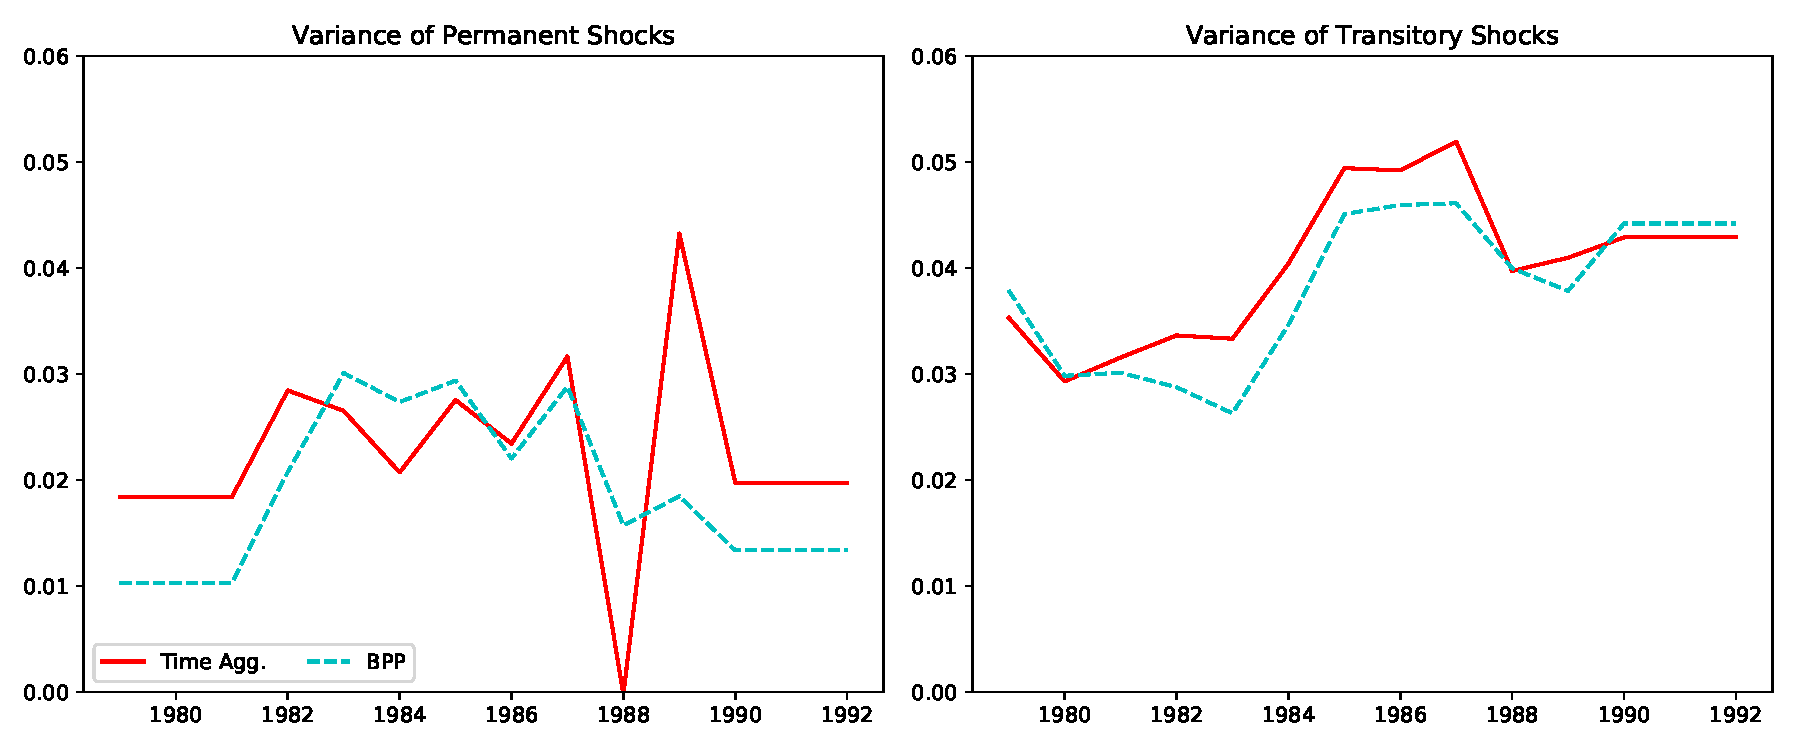
\includegraphics[width=1\textwidth]{Code/Figures/ShockVariances1980s.pdf}
	\footnotesize Notes: BPP plots the variances from Table 6 of the original BPP paper. Time Agg. plots the equivalent variances corrected for the time aggregation problem.
\end{figure}

Table \ref{table:ReplicationTable7} replicates Table 7 from the original BPP paper.

\input Code/Tables/RepTable7.tex

Table \ref{table:ReplicationTable8} replicates Table 8 from the original BPP paper.

\input Code/Tables/RepTable8.tex

\processdelayedfloats

\bibliography{\texname}
% Can't use econtexBibMake because it contains a bibliographystyle command and assumes that \jobname is \texname
%\input econtexBibMake

\pagebreak\appendix
\input AppendixFullMoments.tex
\input AppendixTransitoryPersistence.tex

\end{document}
